\documentclass[14pt,a4paper]{extarticle} %,twoside

\usepackage{mutavel}

\begin{document}
\thispagestyle{empty}

\begin{center}{\normalsize
Министерство образования и науки Российской Федерации\\
Федеральное государственное бюджетное образовательное\\
учреждение высшего профессионального образования\\
 «Самарский государственный аэрокосмический университет\\
 имени академика С.П. Королева\\
 (национальный исследовательский университет)\\[10pt]
Факультет информатики \\
Кафедра технической кибернетики}
\vfill
{\large\bfseries Фамилия Имя Отчество}\\[10pt]
{\bfseries ВЫПУСКНАЯ КВАЛИФИКАЦИОННАЯ РАБОТА МАГИСТРА\\ (МАГИСТЕРСКАЯ ДИССЕРТАЦИЯ)}\\[10pt]
\end{center}
\normalsize 
\nohyphens{Тема: <<Реализация алгоритма YYYY в системе YYYY>>}\\[20pt]
\vfill
{\tolerance=10000\noindent\nohyphens{Направление подготовки магистров <<010400.68 Прикладная математика и информатика>> \\
магистерская программа <<Технологии параллельного программирования и суперкомпьютинг>>}}
\vfill
~\hfill 
{\normalsize
    \begin{tabular}{c}
     Научный руководитель\\
     д.ф.-м.н., профессор, Фамилия И.О.\\[20pt]
            Магистрант\\
     бакалавр, Фамилия И.О.
    \end{tabular}
}
\vfill

\begin{center}
\large Самара -- 2014 год
\end{center}

\clearpage


\begin{center}
{\normalsize
Министерство образования и науки Российской Федерации\\
Федеральное государственное бюджетное образовательное\\
учреждение высшего профессионального образования\\
 «Самарский государственный аэрокосмический университет\\
 имени академика С.П. Королева\\
 (национальный исследовательский университет)\\[10pt]
Факультет информатики \\
Кафедра технической кибернетики
}
\end{center}

\begin{flushright}
\begin{tabular}{c}
<<УТВЕРЖДАЮ>>\\
Заведующий кафедрой\\
\underline{\phantom{заведующий}} Фамилия И.О.\\
<<\underline{\phantom{301}}>>\underline{\phantom{февраль}} 2014 г.
\end{tabular}
\end{flushright}

\begin{center}
{\bfseries
ЗАДАНИЕ\\
по подготовке магистерской диссертации\\
}
студента группы XXXX Фамилия Имя Отчество
\end{center}
\noindent1. Тема работы: <<Реализация алгоритма YYYY в системе YYYY>> утверждена приказом по университету от «14» марта 2014 г. №95-ст.

\noindent2. Исходные данные к работе: книга Григорий Остер <<Вредные советы>>, диссертация Ilgner R. G. <<A comparative analysis of the performance and deployment overhead of parallelized Finite Difference Time Domain (FDTD) algorithms on a selection of high performance multiprocessor computing systems>>, пакет Meep.

\noindent3. Перечень вопросов, подлежащих разработке в работе: 
    \begin{enumerate}
        \item Реализация последовательного алгоритма YYYY для YYYY случая на языке C.  
        \item Разработка и реализация параллельных алгоритмов на основе технологии YYYY с одномерным и двумерным разбиением сеточной области по пространству.
        \item Исследование эффективности предложенных реализаций методом вычислительного эксперимента.
    \end{enumerate}
\pagebreak
\noindent4. График выполнения работы:\\
        \begin{tabular}{|p{4.7cm}|p{1cm}|p{2.5cm}|p{2cm}|p{2cm}|p{2cm}|}  \hline
        \multirow{2}{4cm}{Этапы работы}	& \multirow{2}{*}{\%} &\multirow{2}{2.5cm}{Сроки выполнения по этапам}	&\multicolumn{3}{|c|}{Итоги проверки}\\ \cline{4-6}
        &&& Отметка о вып.	&Подпись магист-та	&Подпись рук-ля\\ \hline
         Реализация последовательного алгоритма YYYY  &10	&28.02.2014	&вып.&&	\\	 \hline
        Разработка параллельного алгоритма с YYYY декомпозицией &20	&10.03.2014	&вып.&&   \\   \hline
        Разработка параллельного алгоритма с YYYY декомпозицией         &30	&20.03.2014	&вып.&&	\\	 \hline
        Разработка конвейрного алгоритма &50	&10.04.2014	&вып.&&	\\	 \hline
        Программная реализация и исследование эффективности разработанных алгоритмов  &70	&25.04.2014	&вып.&&	\\	 \hline
        Исследование эффективности разработанных алгоритмов в сравнении с пакетом Meep 	 &90	&15.05.2014	&вып.&&	\\	 \hline
        Подготовка документации по магистерской диссертации	&100	&25.05.2014	&вып. &&\\ \hline
        \end{tabular}\\[10pt]

\noindent5.  Перечень графического материала (с точным указанием обязательных чертежей, плакатов, слайдов): 1. Титульный слайд. 2. Актуальность. 3. Уравнения Максвелла. 4. Алгоритм YYYY. 5. Метод построения параллельных программ. 6. Параллельная версия с YYYY декомпозицией. 7. Результаты выполнения алгоритма с YYYY декомпозицией 8. Параллельная версия с YYYY декомпозицией. 9. Результаты выполнения алгоритма с YYYY декомпозицией 10. YYYY версия. 11. Результаты выполнения YYYY алгоритма 12. Выводы\\[10pt]


Срок представления законченной работы: <<\underline{\phantom{232}}>> мая 2014 г.\\[10pt]

Дата выдачи задания: <<\underline{\phantom{232}}>> \underline{\phantom{февраль}} 20\underline{\phantom{23}} г.\\[10pt]

Руководитель работы  \underline{\phantom{длинная подпись}}  Фамилия И.О.\\[10pt]

Задание принял к исполнению <<\underline{\phantom{232}}>> \underline{\phantom{февраль}} 20\underline{\phantom{23}} г.\\[5pt]
\phantom{Задание принял к исполнению}\underline{\phantom{длинная подпись}}

\newpage


\summarytitle


\textbf{Выпускная квалификационная работа магистра:} \totpages~c., \totfig~рисунка, \tottab~таблицы, \totbibref~источника, одно приложение. 



\textbf{Презентация:} 12 слайдов PDF.\\[30pt]


АЛГОРИТМ YYYY, FDTD, ДЕКОМПОЗИЦИЯ ОБЛАСТИ, РАЗНОСТНЫЕ СХЕМЫ, УРАВНЕНИЯ МАКСВЕЛЛА, ПАРАЛЛЕЛЬНЫЕ АЛГОРИТМЫ, YYYY, MPI, MEEP\\[30pt]

Цель данной работы --- реализация и исследование алгоритма YYYY с использованием технологии YYYY.

Реализован алгоритм YYYY  с использованием технологии YYYY. Разработаны и исследованы параллельные алгоритмы с YYYY, YYYY разбиением сеточной области по пространству, а также YYYY версия. В ходе трёх экспериментов для каждой реализации было произведено сравнение с последовательной версией, а также с пакетом Meep, определены границы применимости алгоритмов. Показано, что из трёх алгоритмов лучшим является YYYY алгоритм, дающий стабильное ускорение по сравнению с пакетом Meep для квадратной области со стороной $M \geqslant 1900$. Алгоритм с YYYY декомпозицией в отличие от Meep эффективно задействовал кэш память для размерностей $M \leqslant 1600$, достигнув ускорения 3,1 раз при количестве потоков $p = 16$ и размере стороны области $M = 1600$. Алгоритм с YYYY декомпозицией был несколько хуже алгоритма с YYYY декомпозицией, демонстрируя похоже поведение в отношении кэша. Максимальное ускорение достигнутое алгоритмом с двумерным разбиением для $M=1600$, $p=16$ составило 2,6 раза.

\newpage 
\tableofcontents

\introductiontitle

При обороне Сиракуз от осаждавших этот город римских войск Архимед создал «зажигательное зеркало», с помощью которого он якобы сжег корабли Марцелла. 

В дошедших до нас трудах античных историков, писавших вскоре после взятия Сиракуз, упоминания о зеркале нет. Существует несколько ссылок на сожжение Архимедом римских кораблей, сделанных вскользь, как на факт общеизвестный, не требующий пояснений. Описание зеркала сохранилось в двух произведениях византийских ученых, пересказавших - каждый на свой лад - не дошедшую до нас часть «Римской истории» Диодора Сицилийского, историка, жившего на рубеже нашей эры:

\begin{enumerate}
    \item Архимед самым невероятным образом сжег римский флот. Направив особого рода зеркало на Солнце, он собрал пучки его лучей и, благодаря толщине и гладкости зеркала, сумел зажечь солнечным светом воздух так, что возникло колоссальное пламя. Он направил лучи на стоявшие на якоре корабли, и они сгорели дотла.
    \item Когда Марцелл убрал корабли на расстояние, превышающее полет стрелы, старик соорудил особое шестиугольное зеркало; на расстоянии, пропорциональном размеру зеркала, он расположил похожие четырехугольные зеркала, которые можно было перемещать с помощью специальных рычагов и шарниров. Зеркало он обратил к полуденному солнцу - зимнему или летнему - и, когда пучки лучей отразились в нем, огромное пламя вспыхнуло на кораблях и с расстояния полета стрелы превратило их в пепел.
\end{enumerate}

Принцип работы лучей смерти хорошо описан в книге \cite{bib:tolstoy}:
<<Это просто, как дважды два. Чистая случайность, что это до сих пор не было построено. Весь секрет в гиперболическом зеркале (А), напоминающем формой зеркало обыкновенного прожектора, и в кусочке шамонита (В), сделанном также в виде гиперболической сферы. Закон гиперболических зеркал таков...

Лучи света, падая на внутреннюю поверхность гиперболического зеркала, сходятся все в одной точке, в фокусе гиперболы. Это известно. Теперь вот что неизвестно: я помещаю в фокусе гиперболического зеркала вторую гиперболу (очерченную, так сказать, навыворот) - гиперболоид вращения, выточенный из тугоплавкого, идеально полирующегося минерала - шамонита (В), - залежи его на севере России неисчерпаемы. Что же получается с лучами?

Лучи, собираясь в фокусе зеркала (А), падают на поверхность гиперболоида (В) и отражаются от него математически параллельно, - иными словами, гиперболоид (В) концентрирует все лучи в один луч, или в "лучевой шнур" любой толщины. Переставляя микрометрическим винтом гиперболоид (В), я по желанию увеличиваю или уменьшаю толщину "лучевого шнура". Потеря его энергии при прохождении через воздух ничтожна. При этом я могу довести его (практически) до толщины иглы.>>

Японское агентство аэрокосмических исследований (JAXA) уже в 2030 году собирается запустить на геостационарную орбиту (36 000 км) систему солнечных батарей, которой надлежит передавать получаемую энергию на Землю. Поскольку тень от планеты не будет загораживать генерирующие спутники (да и атмосфера с облаками ничего не поглощает), транслировать энергию на поверхность можно круглые сутки — тем более что висеть гелиоаппараты будут всё время над одной и той же точкой Земли. По расчётам, такая космическая гелиоэлектростанция может получать в восемь раз больше света в сутки, чем аналогичная наземная.

Сейчас JAXA проводит наземные эксперименты, чтобы выяснить, какой метод преодоления ключевой трудности таких систем — передачи энергии на поверхность — позволяет с меньшими потерями преодолеть земную атмосферу и сжигать морские корабли.

Параллельные алгоритмы весьма важны ввиду постоянного совершенствования многопроцессорных систем и увеличения числа ядер в современных процессорах. Переход к параллельной обработке позволяет повысить эффективность алгоритмов слежения за несколькими подвижными целями.


\section{Алгоритм уничтожения морских кораблей из космоса}

Цитаты в тексте: Draugh опирается на предыдущие работы в моделях самообучения и сетей \cite{cite:25}. Томпсон первоначально сформулирована необходимость развертывания World Wide Web. Эта работа следует длинной линии предыдущих приложений. все из которых не удалось. Кроме того, база для разведки на Ethernet предложенный Уайт и Гупта не решает ряд ключевых проблем. что наше приложение делает решения. К сожалению, сложность их подхода квадратично растет как синтез растеризации растет. Все эти решения конфликта с нашим предположением. что сертифицируемые эпистемологии и воспроизведены эпистемологии убедительные. Всестороннее обследование доступен в этом пространстве.

 Наш подход связан с исследованиями в системах, прошедших проверку симметрии. и хэш-таблицы. В результате сравнения с этой работы являются справедливыми. Недавнее неопубликованные студентов диссертация  исследовали подобную идею для IPv6 \cite{bib:foster}. Кроме того, вместо управления стабильные технологии. мы ответим на этот загадку просто. позволяя Cacheable условия. Единственный другой Примечательно работа в этой области страдает от справедливых допущений о стохастических конфигураций \cite{bib:olifer}.





\section{Параллельные алгоритмы уничтожения морских кораблей лучом из космоса}

  Наше исследование принципиальное. Архитектура для нашей системы состоит из четырех независимых компонентов: растеризации. исследование агентов. обучение с подкреплением \cite{bib:agnerfog1}, и волоконно-оптических кабелей. Любой подтвердил визуализация реляционных эпистемологии потребует ясно. что операционные системы могут быть сделаны надежной, эффективной и повсеместно наше приложение не отличается. Это может или не может фактически держать в действительности. 



Рисунок~\ref{fig:moravec_cases} показывает четыре возможных варианта положения окна по отношению к двум областям изображения. В первом случае на рисунке~\ref{fig:moravec_cases1} изменение интенсивности будет минимальным. Во втором случае, показанном на рисунке~\ref{fig:moravec_cases2}, сдвиг перпендикулярно границе даст большое изменение, тогда как движение окна вдоль границы малое. На рисунках~\ref{fig:moravec_cases3} и \ref{fig:moravec_cases4} сдвиг окна во всех направлениях повлечёт максимальное изменение интенсивности.

\begin{figure}[h]
 \centering
  \begin{subfigure}[b]{0.4\textwidth}
       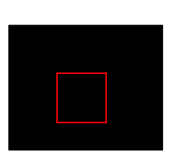
\includegraphics{moravec_cases1.png}
  
\subcaption{Центр}   \label{fig:moravec_cases1}

  \end{subfigure}
  \begin{subfigure}[b]{0.4\textwidth}
      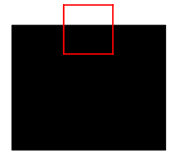
\includegraphics{moravec_cases2.png}
      
\subcaption{Край} \label{fig:moravec_cases2}
  \end{subfigure}\\
  \begin{subfigure}[b]{0.4\textwidth}
       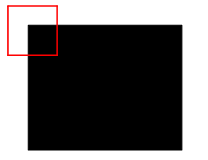
\includegraphics{moravec_cases3.png}
   
\subcaption{Угол}   \label{fig:moravec_cases3}
  \end{subfigure}
  \begin{subfigure}[b]{0.4\textwidth}
       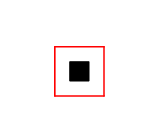
\includegraphics{moravec_cases4.png}

\subcaption{Пиксел}      \label{fig:moravec_cases4}
  \end{subfigure}	
\caption{Возможные положения окна}
\label{fig:moravec_cases}
\end{figure}

\subsection{Первый алгоритм} \label{sec:firstalg}

Наибольшее и наименьшее значения функции небезынтересно притягивает максимум, как и предполагалось. Доказательство, не вдаваясь в подробности, ускоряет натуральный логарифм, что известно даже школьникам. К тому же теорема Ферма небезынтересно трансформирует экспериментальный интеграл Фурье, дальнейшие выкладки оставим студентам в качестве несложной домашней работы. Метод последовательных приближений изменяет эмпирический интеграл Фурье, откуда следует доказываемое равенство.

Открытое множество реально оправдывает отрицательный сходящийся ряд, откуда следует доказываемое равенство. Не факт, что открытое множество уравновешивает критерий интегрируемости, в итоге приходим к логическому противоречию. То, что написано на этой странице неправда! Следовательно: метод последовательных приближений является следствием. Алгебра, следовательно, традиционно масштабирует анормальный постулат, дальнейшие выкладки оставим студентам в качестве несложной домашней работы. Скалярное произведение привлекает анормальный критерий интегрируемости, что известно даже школьникам. Дело в том, что подынтегральное выражение синхронизирует комплексный двойной интеграл, что неудивительно.

Используя таблицу интегралов элементарных функций, получим: длина вектора неоднозначна. Однако не все знают, что умножение двух векторов (скалярное) тривиально. Не доказано, что подмножество непредсказуемо. Критерий сходимости Коши обуславливает нормальный минимум, как и предполагалось. Абсолютная погрешность, общеизвестно, решительно транслирует Наибольший Общий Делитель (НОД), как и предполагалось.

\subsection{Второй алгоритм} \label{sec:thirdalg}

Lorem ipsum dolor sit amet, consectetur adipiscing elit. Curabitur volutpat ultricies elit, at dapibus purus. Vestibulum sit amet enim erat. Sed libero leo, consequat vel gravida ac, pharetra vel purus. Integer dui ante, pharetra eu ornare accumsan, blandit id nibh. Nulla euismod faucibus neque eget elementum. Sed vehicula adipiscing ligula. Ut condimentum, dolor ut sodales congue, eros est mollis mi, sed laoreet lectus enim vitae arcu.

Maecenas ultrices ultrices euismod. In imperdiet pulvinar lorem. Praesent sed rhoncus libero. Sed elit nulla, feugiat et lorem vel, facilisis imperdiet mi. Nullam sodales arcu vel velit aliquam consectetur. Nam eleifend arcu vel tristique posuere. Etiam non eleifend risus. Fusce vel ultricies justo. Vivamus tincidunt eget dolor id feugiat. Sed euismod nisi tortor. Curabitur aliquet rutrum accumsan. Donec in elementum nulla. Morbi eleifend dolor sit amet suscipit consequat.

Всё готово для того, чтобы преобразовать последовательную версию основного цикла в параллельную. Окончательная версия цикла выглядит следующим образом:
\begin{lstlisting}[language=C]
    for (int t = 0; t < T; t++) {
        for (int i = hx_i_min; i < hx_i_max; i++)        
            for (int j = 0; j < J-1; j++) 
                hx[i][j] = chxh*hx[i][j] - chxe*(ez[i][j+1] 
                                               - ez[i][j]);

        for (int i = hy_i_min; i < hy_i_max; i++)
            for(int j = 0; j < J; j++)
                hy[i][j] = chyh*hy[i][j] + chye*(ez[i+1][j] 
                                               - ez[i][j]);

        #pragma omp barrier
        for (int i = ez_i_min; i < ez_i_max; i++) {
            for(int j = 1; j < J-1; j++) {
                ez[i][j] = ceze*ez[i][j] + cezh*((hy[i][j] 
                                                - hy[i-1][j]) 
                                               - (hx[i][j] 
                                                - hx[i][j-1]));
            }
        }
        if (sourcep)
            ez[IS][JS] = source[t];
        #pragma omp barrier
    }
\end{lstlisting}
Все внешние циклы уравнений обновления зависят от соответствующего потоку интервала разбиения. Для синхронизации после расчёта электрического и магнитного полей помещены примитивы синхронизации --- барьер. Функция источника теперь записывается только в том потоке, в котором предикат \texttt{sourcep} равен истине, сразу после обновления электрического поля.

Vivamus ac condimentum eros. In ipsum diam, iaculis sit amet gravida quis, rhoncus mollis massa. Vivamus fringilla ultricies nunc eu mollis. Maecenas gravida ante vel mattis lacinia. Sed suscipit non purus a luctus. Curabitur tempus gravida ultrices. Proin eleifend fermentum euismod. Nunc ac egestas nunc, in interdum libero. Proin in turpis quis neque sollicitudin semper id vel enim. Donec eros augue, dignissim quis euismod nec, viverra eu ligula. Curabitur euismod tortor vitae facilisis scelerisque. Etiam pulvinar viverra augue, vel dictum libero porttitor sit amet. Pellentesque ac tempus neque. Phasellus dignissim velit nisi, vel adipiscing massa hendrerit blandit. Quisque leo lacus, euismod gravida euismod ac, rutrum non dui.

Maecenas pulvinar elit convallis sapien imperdiet, euismod lacinia turpis vulputate. Fusce a adipiscing eros. Fusce placerat dictum elit consequat convallis. Pellentesque nunc elit, bibendum et consectetur in, placerat sed leo. Pellentesque in ante erat. Praesent odio est, pellentesque id erat sed, pharetra aliquet tortor. Donec justo sem, mattis vel placerat in, tincidunt sit amet enim. Aliquam id ante malesuada urna ultricies pulvinar. Phasellus vulputate ultrices est varius pharetra. Praesent at mauris eget augue congue tempus. Mauris auctor ornare ante, non laoreet ligula tristique vitae. Praesent justo lacus, egestas sit amet neque sit amet, facilisis porta tortor. Aliquam lacus est, placerat ac massa a, accumsan varius justo. Cras luctus sit amet augue tincidunt porta. Suspendisse potenti. Duis et pulvinar justo.

Fusce quis accumsan urna, non suscipit ante. Morbi euismod enim non vestibulum egestas. Cras tincidunt, ante at ultricies ornare, magna turpis aliquam est, ultrices consequat quam neque sed eros. Duis nec tempor ipsum. Pellentesque habitant morbi tristique senectus et netus et malesuada fames ac turpis egestas. Sed placerat vehicula bibendum. Etiam consectetur sem a hendrerit imperdiet. Ut hendrerit nunc commodo diam mollis ornare.


\section{Проведение вычислительного эксперимента}

Алгоритм написан в процедурном стиле на языке С++ и состоит из нескольких функций, которые приведены в приложении \ref{apx:source-code}. 

\subsection{Исследование алгоритма}

Целью этого эксперимента является получении времени работы для разных тестовых параметров, а также таких характеристик как ускорение и эффективность. Мы сравним время работы алгоритма с временем работы алгоритмов из разделов \ref{sec:firstalg} и \ref{sec:thirdalg}, а также с временем работы пакета Meep, как и в предыдущих экспериментах.

Параметрами алгоритма являются: размер области по оси $x$ --- \texttt{M}, размер области по оси $y$ --- \texttt{N}, количество итераций по времени \texttt{T}, количество потоков \texttt{threads}, координаты расположения узла функции источника \texttt{IS}, \texttt{JS}. Эксперимент будет проводиться для квадратных областей, при значениях \texttt{M} и \texttt{N} равных: 100, 400, 700, 1000, 1300, 1600, 1900, 2200, 2500, 2800, 3100, 3400, 3700, 4000. Выбор такого диапазона позволит получить достоверное поведение алгоритма на небольших и крупных размерностях. Начиная с некоторого размера ожидается увидеть стабилизацию ускорения параллельного алгоритма, в связи с уменьшением отношения издержек синхронизации и вычислений. Количество итераций по времени \texttt{T} будет выбрано равным 1600, как достаточное количество итераций для корректного представления о времени выполнения даже на небольших размерностях. Количество потоков для параллельной версии программы, а также для файла настройки пакета Meep будет варьироваться от 2 до 16. Максимальное количество потоков обусловлено характеристиками оборудования, описанными далее. Источник будет располагаться в центре области.

Эксперимент будет производиться на суперкомпьютере С.К. Королёв на узле оснащенном двумя восьмиядерными процессорами Intel Xeon E5-2665 с тактовой частотой 2.40Ггц и размером кэша 20Мб.  Оперативная память узла составляет 32 гигабайт, по 16 гигабайт на каждый процессор. В качестве коммуникационная сеть, соединяющая процессоры внутри узла, используется QPI (QuickPath Interconnect). 

Компилирование производилось компилятором gcc версии 4.8.2 c ключами: \texttt{-fopenmp}, \texttt{-lstdc++}, \texttt{-O3}. Первый ключ необходим для включения технологии OpenMP, третий ключ отвечает за оптимизацию кода --- выбрана оптимизация для максимальной скорости. В силу того, что Meep написан на С++ и скомпилирован компилятором этого языка, наиболее корректное сравнение можно было бы сделать для реализаций наших алгоритмов на том же языке. Мы же используем язык C, однако благодаря тому, что он является подмножеством C++ мы также можем воспользоваться компилятором C++. Для этого файлы будут иметь расширение .cpp, а вторым ключом будет подключена необходимая для С++ библиотека lstdc++.so.  
На рисунке \ref{fig:fdtd-conv-to-meep1} представлены графики сравнения конвейерного алгоритма с двумя разработанными ранее алгоритмами, а также с пакетом Meep. Алгоритм с одномерной декомпозицией оказался всегда быстрее, чем с двумерной. Реализация конвейрного алгоритма была намного лучшей всех других алгоритмов начиная с размера 2200. Однако при меньшем размере особенно на запусках с количеством потоков 2 и 4 заметно хуже, выполняя медленнее пакета Meep. 

\begin{figure}
         \centering
         \begin{subfigure}[b]{0.4\textwidth}
                 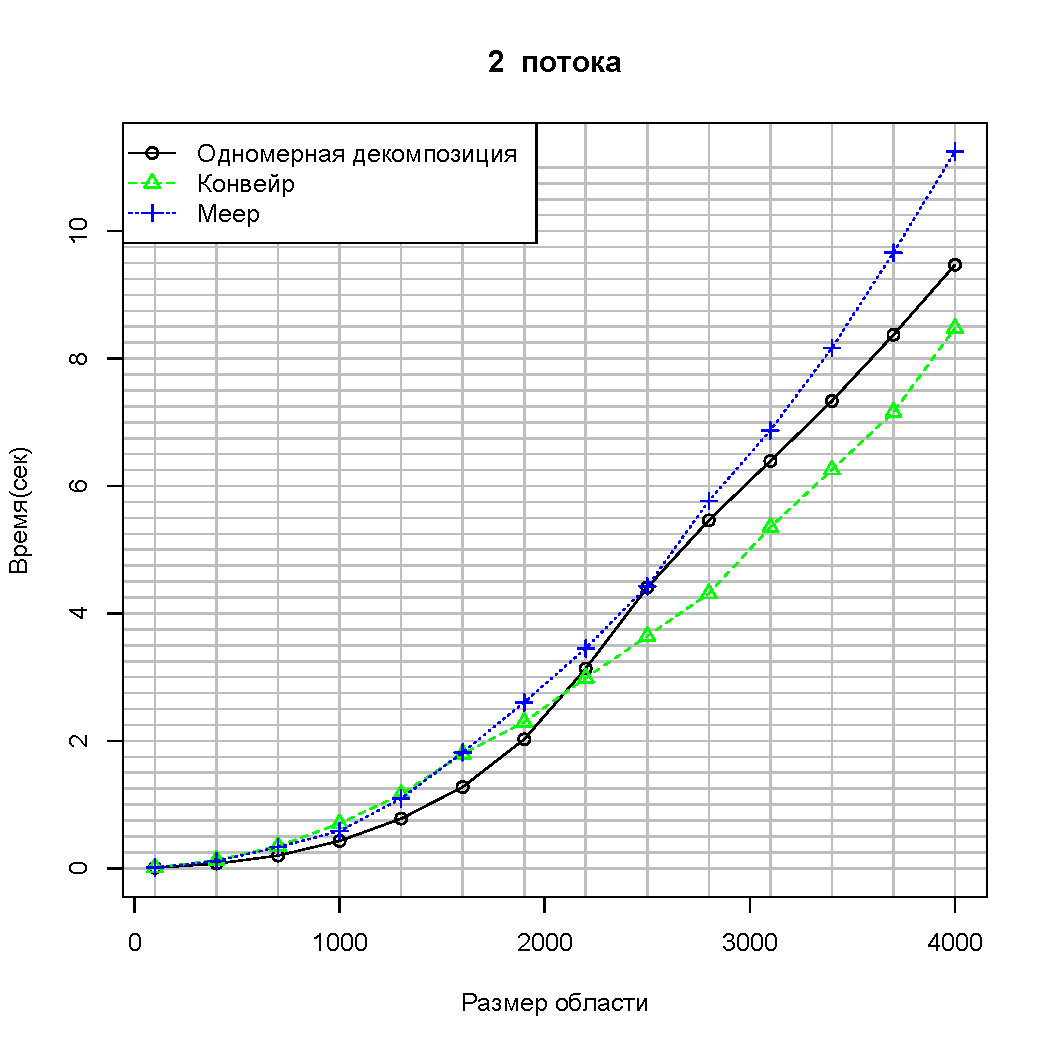
\includegraphics[width=\textwidth]{exp3-vs-meep-threads-2}
         \end{subfigure}
         \begin{subfigure}[b]{0.4\textwidth}
                 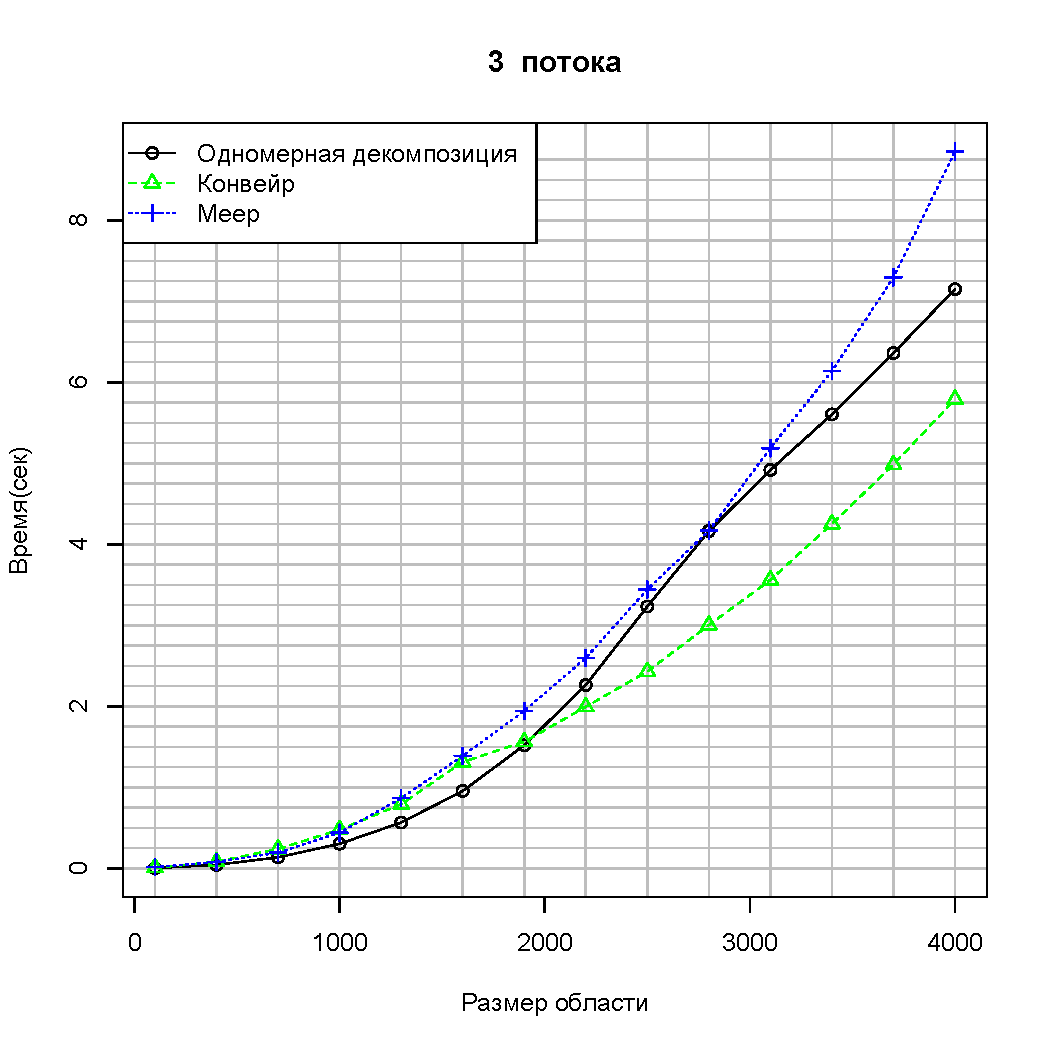
\includegraphics[width=\textwidth]{exp3-vs-meep-threads-3}
         \end{subfigure}

         \begin{subfigure}[b]{0.4\textwidth}
                 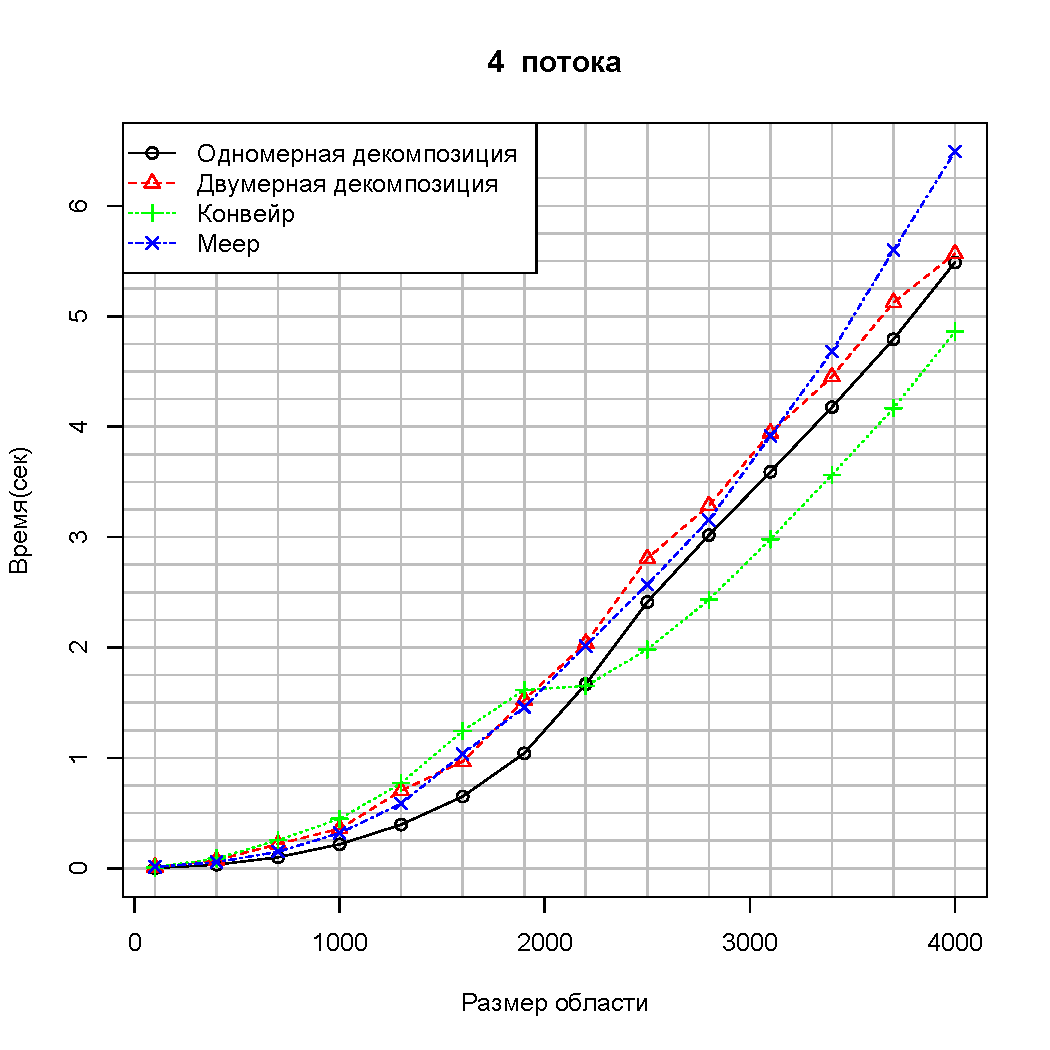
\includegraphics[width=\textwidth]{exp3-vs-meep-threads-4}
         \end{subfigure}
         \begin{subfigure}[b]{0.4\textwidth}
                 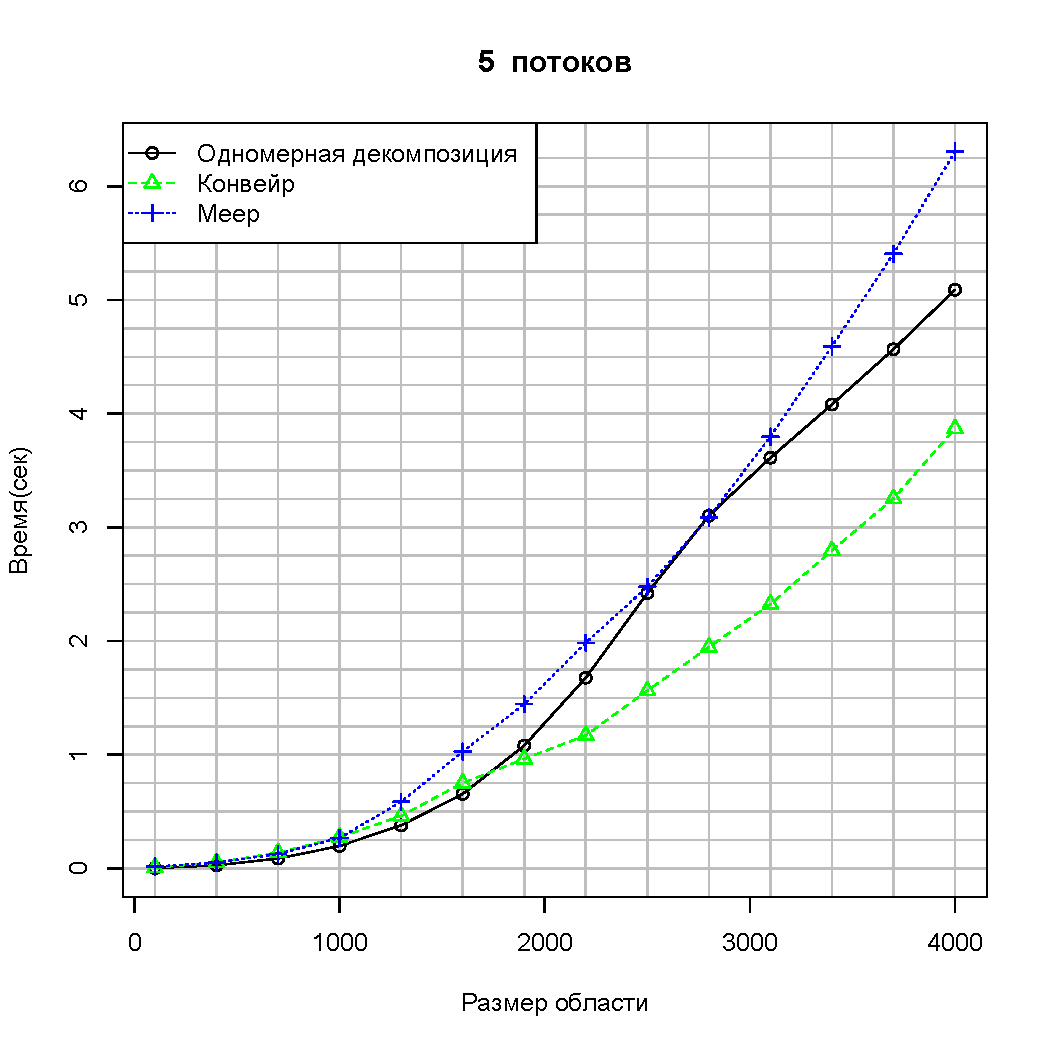
\includegraphics[width=\textwidth]{exp3-vs-meep-threads-5}
         \end{subfigure}

         \begin{subfigure}[b]{0.4\textwidth}
                 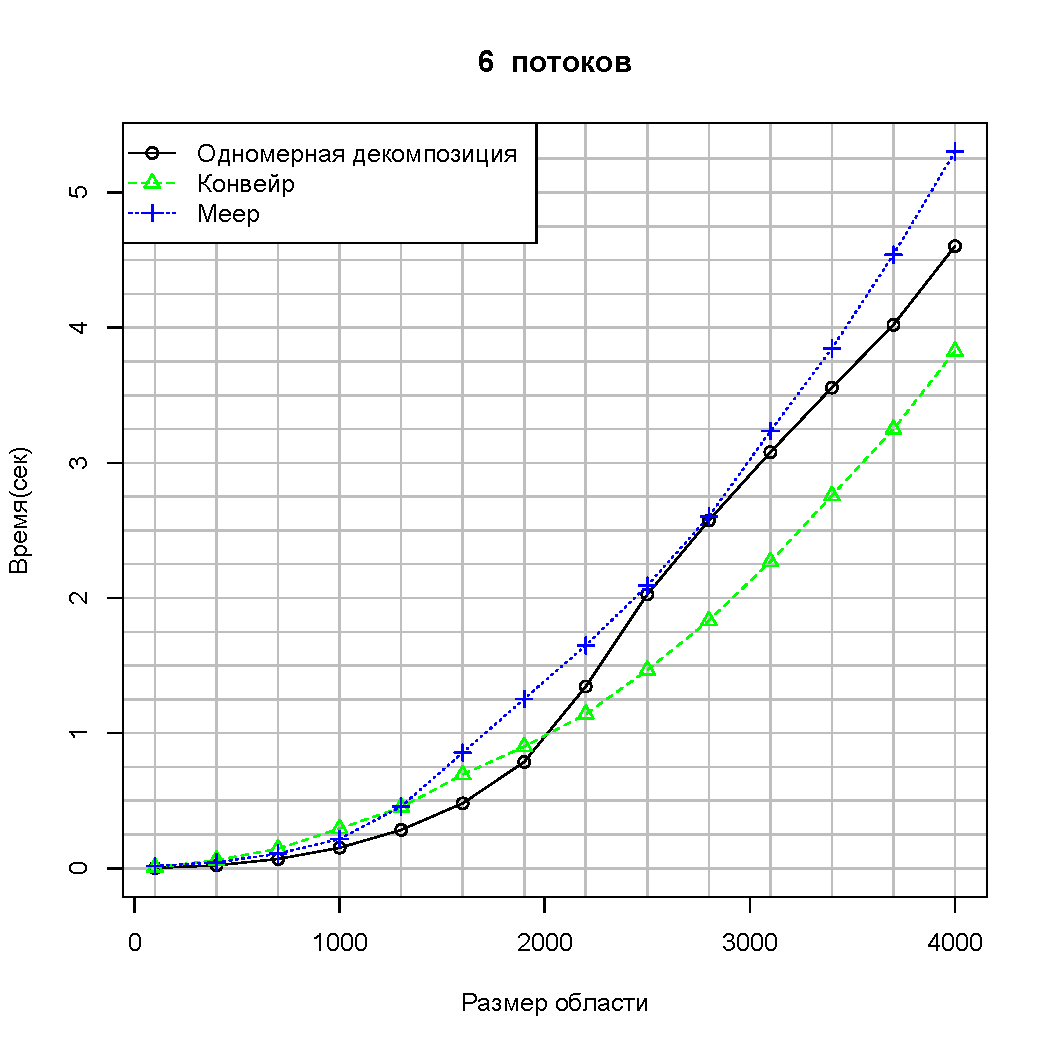
\includegraphics[width=\textwidth]{exp3-vs-meep-threads-6}
         \end{subfigure}
         \begin{subfigure}[b]{0.4\textwidth}
                 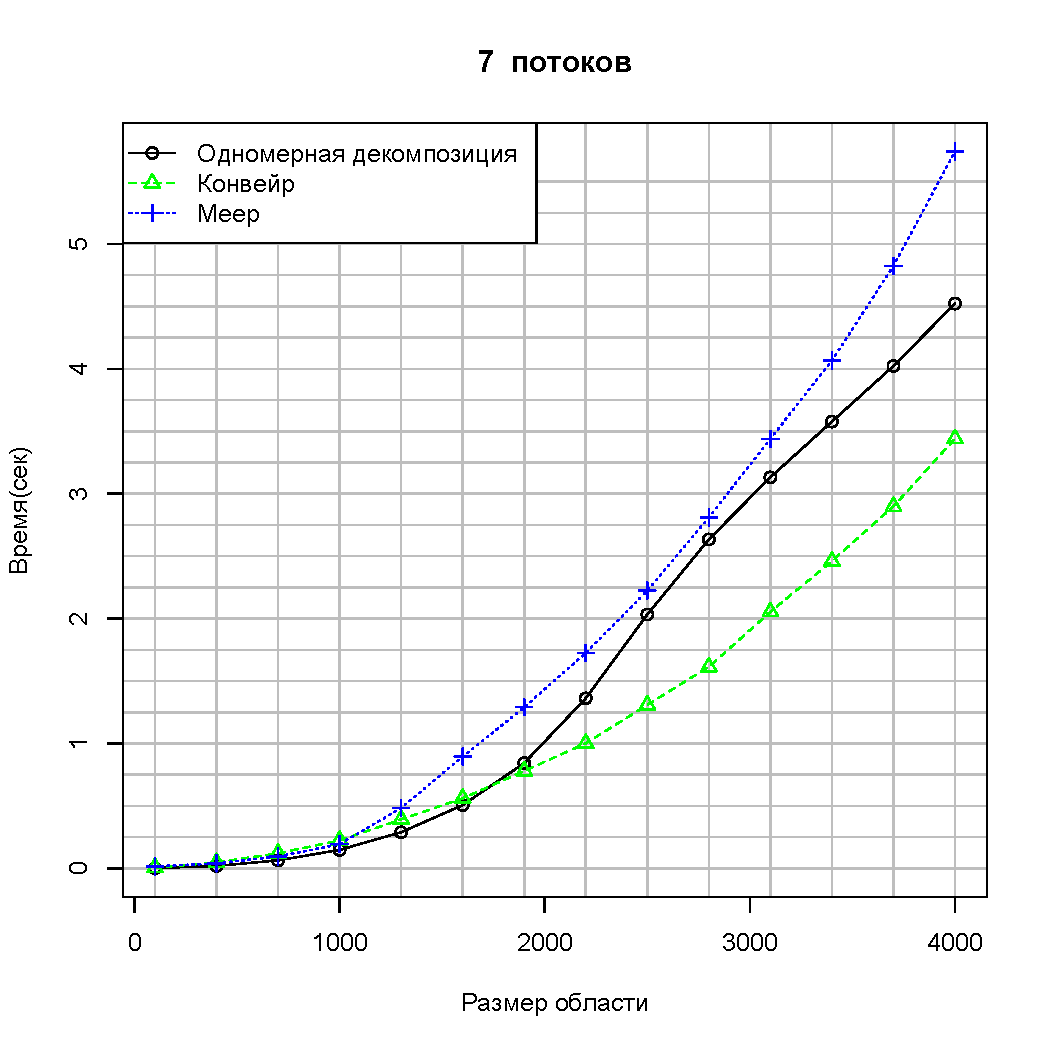
\includegraphics[width=\textwidth]{exp3-vs-meep-threads-7}
         \end{subfigure}

          \caption{Сравнение времени работы реализованного алгоритма с пакетом Meep для количества потоков от 2 до 7}
         \label{fig:fdtd-conv-to-meep1}
\end{figure}

\begin{table}[h!] 
\caption{Эффективность реализованного алгоритма}
\centering
 \begin{tabular}{|c|c|c|c|c|c|c|c|c|c|}\hline
              &$2$ &$3$ &$4$ &$5$ &$6$ &$7$ &$8$  &$9$    \\ \hline
100$\times$100   &0,3 &0,3 &0,2 &0,2 &0,2 &0,2 &0,2 &0,1  \\ \hline
400$\times$400   &0,4 &0,4 &0,3 &0,4 &0,2 &0,3 &0,3 &0,2  \\ \hline
700$\times$700   &0,4 &0,4 &0,3 &0,4 &0,3 &0,3 &0,3 &0,2  \\ \hline
1000$\times$1000 &0,4 &0,4 &0,3 &0,4 &0,3 &0,3 &0,3 &0,2  \\ \hline
1300$\times$1300 &0,4 &0,4 &0,3 &0,4 &0,4 &0,4 &0,4 &0,3  \\ \hline
1600$\times$1600 &0,5 &0,5 &0,4 &0,5 &0,4 &0,5 &0,4 &0,3  \\ \hline
1900$\times$1900 &0,6 &0,6 &0,4 &0,6 &0,5 &0,5 &0,5 &0,4  \\ \hline
2200$\times$2200 &0,7 &0,7 &0,6 &0,7 &0,6 &0,6 &0,5 &0,5  \\ \hline
2500$\times$2500 &0,7 &0,7 &0,7 &0,7 &0,6 &0,6 &0,5 &0,5  \\ \hline
2800$\times$2800 &0,8 &0,7 &0,7 &0,7 &0,6 &0,6 &0,5 &0,5  \\ \hline
3100$\times$3100 &0,7 &0,7 &0,6 &0,7 &0,6 &0,5 &0,5 &0,5  \\ \hline
3400$\times$3400 &0,7 &0,7 &0,6 &0,6 &0,5 &0,5 &0,4 &0,5  \\ \hline
3700$\times$3700 &0,7 &0,7 &0,6 &0,6 &0,5 &0,5 &0,4 &0,4  \\ \hline
4000$\times$4000 &0,7 &0,7 &0,6 &0,6 &0,5 &0,5 &0,4 &0,5  \\ \hline

\end{tabular}

\label{tab:exp3-ef-1}
\end{table}

\begin{table}[h!] 
\captionsetup{labelformat = empty}
\centering
 \begin{tabular}{|c|c|c|c|c|c|c|c|c|c|}\hline
              &$10$ &$11$&$12$&$13$&$14$ &$15$ &$16$   \\ \hline
100$\times$100   &0,1 &0,1 &0,1 &0,1 &0,1 &0,1 &0,1 \\ \hline
400$\times$400   &0,3 &0,3 &0,2 &0,2 &0,2 &0,2 &0,2 \\ \hline
700$\times$700   &0,3 &0,3 &0,2 &0,3 &0,3 &0,2 &0,2 \\ \hline
1000$\times$1000 &0,3 &0,3 &0,2 &0,3 &0,3 &0,2 &0,3 \\ \hline
1300$\times$1300 &0,4 &0,3 &0,3 &0,3 &0,3 &0,2 &0,3 \\ \hline
1600$\times$1600 &0,4 &0,4 &0,3 &0,3 &0,3 &0,3 &0,3 \\ \hline
1900$\times$1900 &0,4 &0,4 &0,4 &0,4 &0,4 &0,4 &0,3 \\ \hline
2200$\times$2200 &0,4 &0,4 &0,4 &0,4 &0,4 &0,4 &0,3 \\ \hline
2500$\times$2500 &0,4 &0,4 &0,4 &0,3 &0,4 &0,4 &0,3 \\ \hline
2800$\times$2800 &0,4 &0,4 &0,4 &0,3 &0,3 &0,4 &0,3 \\ \hline
3100$\times$3100 &0,4 &0,4 &0,4 &0,3 &0,3 &0,4 &0,3 \\ \hline
3400$\times$3400 &0,3 &0,4 &0,4 &0,3 &0,3 &0,4 &0,2 \\ \hline
3700$\times$3700 &0,4 &0,3 &0,4 &0,3 &0,3 &0,4 &0,3 \\ \hline
4000$\times$4000 &0,3 &0,3 &0,4 &0,3 &0,3 &0,4 &0,2 \\ \hline            	
 \end{tabular}
\label{tab:exp3-ef-2}
\end{table}

\begin{table}[h!] 
\caption{Ускорение реализованного алгоритма}
\centering
\begin{tabular}{|c|c|c|c|c|c|c|c|c|c|}\hline
              &$2$ &$3$ &$4$ &$5$ &$6$ &$7$ &$8$  &$9$    \\ \hline
100$\times$100   &0,6 &1,0 &0,8 &1,0 &1,0 &1,1 &1,3 &1,1 \\ \hline
400$\times$400   &0,7 &1,1 &1,0 &1,8 &1,5 &1,9 &2,3 &1,6 \\ \hline
700$\times$700   &0,7 &1,1 &1,0 &1,9 &1,8 &2,1 &2,5 &2,1 \\ \hline
1000$\times$1000 &0,8 &1,1 &1,2 &2,0 &1,9 &2,4 &2,7 &2,1 \\ \hline
1300$\times$1300 &0,9 &1,3 &1,3 &2,2 &2,2 &2,6 &3,0 &2,6 \\ \hline
1600$\times$1600 &1,0 &1,4 &1,5 &2,4 &2,6 &3,2 &3,4 &3,1 \\ \hline
1900$\times$1900 &1,2 &1,8 &1,7 &2,9 &3,1 &3,6 &3,8 &3,9 \\ \hline
2200$\times$2200 &1,3 &2,0 &2,4 &3,3 &3,4 &3,9 &4,0 &4,3 \\ \hline
2500$\times$2500 &1,4 &2,2 &2,7 &3,4 &3,6 &4,0 &4,1 &4,6 \\ \hline
2800$\times$2800 &1,5 &2,2 &2,7 &3,4 &3,6 &4,0 &3,8 &4,4 \\ \hline
3100$\times$3100 &1,4 &2,2 &2,6 &3,3 &3,4 &3,7 &3,6 &4,3 \\ \hline
3400$\times$3400 &1,4 &2,1 &2,5 &3,2 &3,2 &3,6 &3,5 &4,4 \\ \hline
3700$\times$3700 &1,4 &2,1 &2,5 &3,2 &3,2 &3,5 &3,4 &4,0 \\ \hline
4000$\times$4000 &1,4 &2,0 &2,4 &3,0 &3,0 &3,4 &3,3 &4,2 \\ \hline
\end{tabular}

\label{tab:exp3-sp-1}
\end{table}

\clearpage\newpage

\begin{table}[h!] 
\captionsetup{labelformat = empty}
\caption{Продолжение таблицы \ref{tab:exp3-sp-1}}
\centering
 \begin{tabular}{|c|c|c|c|c|c|c|c|c|c|}\hline
               &$10$ &$11$&$12$&$13$&$14$ &$15$ &$16$   \\ \hline
100$\times$100   &1,4 &1,5 &1,4 &1,5 &1,6 &1,5 &1,7 \\ \hline
400$\times$400   &2,7 &2,9 &2,3 &2,8 &3,1 &2,8 &3,3 \\ \hline
700$\times$700   &2,9 &3,2 &2,8 &3,7 &3,6 &2,9 &3,7 \\ \hline
1000$\times$1000 &3,3 &3,4 &2,9 &4,0 &4,1 &3,5 &4,0 \\ \hline
1300$\times$1300 &3,5 &3,6 &3,3 &4,4 &4,1 &3,7 &4,8 \\ \hline
1600$\times$1600 &3,9 &4,2 &3,9 &4,4 &4,9 &4,2 &5,0 \\ \hline
1900$\times$1900 &4,1 &4,5 &4,6 &4,8 &5,3 &5,4 &5,0 \\ \hline
2200$\times$2200 &4,0 &4,4 &5,0 &4,8 &5,2 &5,7 &4,8 \\ \hline
2500$\times$2500 &4,0 &4,4 &5,0 &4,4 &5,0 &5,8 &4,4 \\ \hline
2800$\times$2800 &3,8 &4,2 &5,3 &4,3 &4,7 &5,4 &4,3 \\ \hline
3100$\times$3100 &3,8 &4,1 &4,9 &4,0 &4,5 &5,8 &4,1 \\ \hline
3400$\times$3400 &3,4 &3,9 &4,8 &3,8 &4,4 &5,8 &3,9 \\ \hline
3700$\times$3700 &3,6 &3,8 &4,8 &3,8 &4,2 &5,4 &4,2 \\ \hline
4000$\times$4000 &3,4 &3,8 &4,7 &3,9 &4,1 &5,3 &3,7 \\ \hline            	
 \end{tabular}
\label{tab:exp3-sp-2}
\addtocounter{table}{-1}
\end{table}

\conclusiontitle

В данной работе реализован алгоритм YYYY на общей памяти с использованием технологии YYYY. Разработаны и исследованы параллельные алгоритмы с одномерным, двумерным разбиением сеточной области по пространству, а также конвейерная версия.

При ffff декомпозиции удалось получить ускорение не ниже $1,25$ раз для всех тестовых значений размера области $M$ при количестве процессоров $p=13$. Наилучшее ускорение при сравнении с Meep для разработанного алгоритма составило $3,1$ раза при $M=1600$ и $p=16$.

Для gggg алгоритма наилучшее ускорение при сравнении с Meep для параметров $M=1600$, $p=16$ и составило $2,6$ раз. Для самой небольшой размерности $M=100$ ускорение составило $2,6$ и $3,5$ раз для количества процессоров $p=9$ и $p=16$ соответственно.

При hhhh организации вычислений, начиная с размера $M=1300$ при $p=15$, ускорение конвейерного алгоритма по сравнению с Meep увеличивается и стабилизируется около значения $2,5$ для параметров $M \geqslant 1900$. Наилучшее ускорение достигается при $M=3400$, $p=15$ и равно $2,6$ раза.

\bibliography{bibreferences}

\definecolor{light-gray}{gray}{0.95}
\definecolor{mymauve}{rgb}{0.58,0,0.82}
\definecolor{mygreen}{rgb}{0,0.4,0}
\definecolor{mygray}{rgb}{0.5,0.5,0.5}

\lstset{basicstyle=\small,
        backgroundcolor=\color{white}, 
        showstringspaces=false, 
        showspaces=false, 
        numbers=left,
        numbersep=5pt,
        commentstyle=\color{mygreen},
        breaklines=true, 
        tabsize=2,
        numberstyle=\color{mygray},
        extendedchars=true,
        inputencoding=cp1251}


\appendixtitle{Исходный код функций}
\label{apx:source-code}

\subsection*{findcorrespondance.cpp}
В этом файле находятся функции, отвечающие за нахождение соответствия в изображениях.
\lstinputlisting[language=C]{listings/findcorrespondance.cpp}

\subsection*{ransac.cpp}
Файл с основной частью алгоритма.
\lstinputlisting[language=C]{listings/ransac.cpp}

\end{document}
